
\section{椭圆初步}
\label{sec:oval-preliminary-discussion}

椭圆曲线形状优雅,方程优美,性质优酷\footnote{又美又酷。}...... 拜托我不能再吹下去了,不然全世界的汽车车轮都该改成椭圆形了,想象一下坐在这样的车上是什么感受......

本节所谓的标准椭圆是指方程为$\frac{x^2}{a^2}+\frac{y^2}{b^2}=1(a>b>0)$的椭圆。

\subsection{焦半径公式}
\label{sec:oval-focal-radius}

椭圆上任一点与焦点的连线称为焦半径,在标准椭圆上任取一点$P(x_0,y_0)$,那么它到左准线的距离$d=x_0+\frac{a^2}{c}$,根据第二定义,它到左焦点$F_1$的距离是$PF_1=ed=a+ex_0$,再根据第一定义,它到右焦点的距离是$PF_2=2a-PF_1=a-ex_0$,于是得坐标形式的 \emph{焦半径公式}:
\begin{equation}
  \label{eq:oval-focal-radius-in-xy}
  PF_1=a+ex_0, \  PF_2=a-ex_0
\end{equation}

\begin{figure}[htbp]
  \centering
\includegraphics{content/analytic-geometry/pic/focal-radius-of-ellipse.pdf}
\caption{椭圆的焦半径}
\label{fig:focal-radius-of-ellipse}
\end{figure}

假定向量$\vv{F_1P}$与$x$轴正方向单位向量成角$\theta$,记其模$r=|\vv{F_1P}|$在$\triangle PF_1F_2$中使用余弦定理可得$(2a-r)^2=r^2+4c^2-4cr\cos{\theta}$,解得
\begin{equation}
  \label{eq:oval-focal-radius-theta}
  r=\frac{b^2}{a-c\cos{\theta}}
\end{equation}
这是倾斜角形式的 \emph{焦半径公式}。

\begin{example}
 如果$PF_1$延长线与椭圆相交于另一点$Q$,易知向量$\vv{F_1Q}$与$x$轴正方向单位向量成角$\theta+\pi$,因此在上式中将$\theta$换成$\theta+\pi$,即得可知
\begin{equation}
  \label{eq:oval-focal-radius-theta-2}
  F_1P=\frac{b^2}{a-c\cos{\theta}}, \  F_1Q=\frac{b^2}{a+c\cos{\theta}}
\end{equation}
从上式立刻得出,如果过焦点$F$的直线与椭圆相交于$P$、$Q$两点,那么有
\begin{equation}
  \label{eq:oval-focal-line-split}
  \frac{1}{FP}+\frac{1}{FQ}=\frac{2a}{b^2}
\end{equation}
\end{example}

\begin{example}
设$A$、$B$是椭圆上的两个动点,且两个动点在运动过程中始终保持$AF_1 \parallel BF_2$,我们来确定$AF_2$与$BF_1$的交点$P$的轨迹。

\begin{figure}[htbp]
  \centering
\includegraphics{content/analytic-geometry/pic/oval-two-focus-radius-intersectionpoint.pdf}
\caption{}
\label{fig:oval-two-focus-radius-intersectionpoint}
\end{figure}

如图 \ref{fig:oval-two-focus-radius-intersectionpoint},假定$AF_1=r_1$,$BF_2=r_2$,由$\triangle PAF_1 \sim \triangle PBF_2$且相似比为$r_1/r_2$,有
\begin{eqnarray*}
  PF_1 + PF_2 & = & \frac{PF_1}{BF_1}BF_1 + \frac{PF_2}{AF_2}AF_2 \\
              & = & \frac{r_1}{r_1+r_2}BF_1 + \frac{r_2}{r_1+r_2}AF_2 \\
              & = & \frac{r_1}{r_1+r_2}(2a-r_2) + \frac{r_2}{r_1+r_2}(2a-r_1) \\
              & = & 2a - \frac{2r_1r_2}{r_1+r_2} \\
              & = & 2a - \frac{2}{\frac{1}{r_1}+\frac{1}{r_2}} \\
  & = & 2a - \frac{b^2}{a}
\end{eqnarray*}
最后一个等号处利用了上一个例子中的结论($BF_2$平行且等于$AF_1$延长后与椭圆相交的另一段线段),这结果这表明点$P$的轨迹是一个具有相同焦点的椭圆。
\end{example}

\subsection{第一定义与第二定义的等价性}
\label{sec:the-equalance-for-two-definition-of-oval}

椭圆两个定义的等价性其实从根据各自的定义得出相同的椭圆方程就可以看出,但这里感兴趣的是纯几何角度的证明,这只要证明下面这个命题就可以了:
\begin{statement}
设$a$和$c$是两个正实数,且$a>c$,$F_1$和$F_2$是平面上相距为$2c(c>0)$的两个定点,$O$为它们的中点,$L$为射线$OF_1$上满足$OL=\frac{a^2}{c}$的点(由于$\frac{a^2}{c}>c$,因此$L$比$F_1$距离$O$更远一些),直线$l$过点$L$且与直线$F_1F_2$垂直,则平面上的动点$P$到$F_1$、$F_2$的距离之和为$2a$的充分必要条件是$\frac{PF_1}{d}=\frac{c}{a}$,其中$d$是动点$P$到直线$l$的距离。
\end{statement}

\begin{figure}[htbp]
  \centering
\includegraphics{content/analytic-geometry/pic/two-definition-of-ellipse.pdf}
\caption{椭圆的第一定义与第二定义}
\label{fig:two-definition-of-ellipse}
\end{figure}

\begin{proof}[证明]
 先证必要性。设直线$PF_1$的倾斜角为$\theta$,记$PF_1=r$,则$PF_2=2a-r$,在三角形$PF_1F_2$中由余弦定理得
\[ (2a-r)^2=r^2+(2c)^2-2r \cdot 2c \cdot \cos{\theta} \]
记$b^2=a^2-c^2$,则由上式解得
\begin{equation}
\label{eq:focal-radius}
r=\frac{b^2}{a-c\cos{\theta}}
\end{equation}

另外,根据几何关系显然有
\begin{equation}
  \label{eq:oval-two-definition-d}
 d=LF_1+PF_1\cos{\theta}=\frac{a^2}{c}-c+r\cos{\theta}=\frac{b^2}{c}+r\cos{\theta} 
\end{equation}
因此
\[ \frac{d}{r}=\frac{1}{r}\frac{b^2}{c}+\cos{\theta} \] 
将式\ref{eq:focal-radius}代入上式右端,立即得到$\frac{d}{r}=\frac{a}{c}$,必要性得证。

下证充分性,倾斜角及$r$的定义同前,此时式\ref{eq:oval-two-definition-d}仍然成立,因此
\[ \frac{a}{c}=\frac{d}{r}=\frac{b^2}{c} \cdot \frac{1}{r}+\cos{\theta} \]
解出$r$即得到\ref{eq:focal-radius},由此之前的余弦定理式也是成立的,因此必然$PF_2=2a-r$,充分性得证。
\end{proof}

\subsection{切线与光学性质}
\label{sec:oval-tangent}

椭圆曲线将其所在平面分成了三个部分:椭圆内部、椭圆曲线上、椭圆外部,对于椭圆曲线上的点,正如大家所熟知的,它们的坐标都满足椭圆的方程:
\begin{equation}
\frac{x^2}{a^2}+\frac{y^2}{b^2}=1 \label{eq:ellipse}
\end{equation}
而对于椭圆内部的点,它们的坐标都满足不等式:
\begin{equation}
\frac{x^2}{a^2}+\frac{y^2}{b^2}<1 \label{neq:innerellipse}
\end{equation}
这个很好理解,对于椭圆内部任何一点,总能在椭圆上找到一个对应点,使其横坐标相同而纵坐标的绝对值大于椭圆内的点,而椭圆曲线上的这个对应点的坐标满足方程\ref{eq:ellipse},那么椭圆内的点的坐标满足不等式\ref{neq:innerellipse}就是显然的事情了。
至于椭圆外部的点,那就只有成立不等式:
\begin{equation}
\frac{x^2}{a^2}+\frac{y^2}{b^2}>1 \label{neq:outerellipse}
\end{equation}
因为之前椭圆曲线与其方程之间以及椭圆内部的平面区域与其不等式之间都是可以互推的。

接下来讨论椭圆的切线问题,所谓切线,仿照圆的定义,按照直线与椭圆的交点数目,把直线与椭圆的位置关系划分为三类:相切、相交、相离。

在椭圆上任取一个点 $P(x_0,y_0)$,我们在例\ref{ep:the-tangent-after-scale-translation}中利用伸缩变换曾经得出过如下的切线方程:
\begin{equation}
\frac{x_0x}{a^2}+\frac{y_0y}{b^2}=1 \label{eq:tangent}
\end{equation}
\begin{center}
%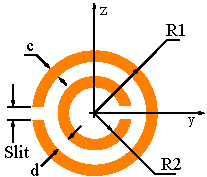
\includegraphics{fig1.png}
\end{center}

\begin{figure}[htbp]
  \centering
\includegraphics{content/analytic-geometry/pic/oval-tangent-line.pdf}
\caption{椭圆的切线}
\label{fig:oval-tangent-line}
\end{figure}

在这里,我们换一个角度来阐明它就是切线,在这直线上任取一点 $T(x_T,y_T)$,有:
\begin{equation}
(\frac{x_0^2}{a^2}+\frac{y_0^2}{b^2})+(\frac{x_T^2}{a^2}+\frac{y_T^2}{b^2}) \geqslant 2(\frac{x_0x_T}{a^2}+\frac{y_0y_T}{b^2})=2
\end{equation}
所以得到:
\begin{equation}
\frac{x_T^2}{a^2}+\frac{y_T^2}{b^2} \geqslant 1
\end{equation}
这表明直线\ref{eq:tangent}上除点$P$外任何一点都在椭圆外,与椭圆只有$P$一个交点,所以它理所当然就是点$P$处的切线方程。

椭圆具有一个漂亮的光学性质:从椭圆的焦点之一发出的光线,经椭圆反射之后,必经过另一个焦点。需要说明的是光线经椭圆反射,等同于经椭圆上相应点处的切线反射。

为着证明这一点,提出如下定理:
\begin{theorem}[椭圆切线定理]
  椭圆上某点处的切线,是该点与椭圆两个焦点连线所形成的焦点三角形在该点处的外角平分线。
\end{theorem}

\begin{proof}[证明]
  分两步证明,先证明定理中所说的外角平分线是椭圆的切线,再证明切线的唯一性。

\begin{figure}[htbp]
  \centering
\includegraphics{content/analytic-geometry/pic/oval-focus-triangle-external-bisector.pdf}
\caption{三角形外角平分线的一个性质}
\label{fig:oval-focus-triangle-external-bisector}
\end{figure}

  要证明此外角平分线与椭圆相切,只需证明它与椭圆只有唯一公共点即可。这实际上来自于平面几何中的一个结论:如图\ref{fig:oval-focus-triangle-external-bisector},点$P$是三角形$\triangle ABC$在顶点$A$处的外角平分线上异于点$A$的任意一点,那么有不等式$PB+PC>AB+AC$成立。

  证明也很简单,作出点$C$关于此外角平分线的对称点$C'$,那么有$PB+PC=PB+PC' > BC' = AB + AC' = AB+AC$.

  这表明点$P$不可能在椭圆上,所以此外角平分线与椭圆除点$A$外无其它公共点,即为切线。

  再继续证明切线的唯一性,这只要证明在上述三角形$ABC$中,过点$A$的其它直线上,必存在另一个异于点$A$的点$Q$,使得$QB+QC=AB+AC$即可,因为这样点$Q$就是该直线与椭圆的另一个交点,从而直线与椭圆是相交而非相切。

\begin{figure}[htbp]
  \centering
\includegraphics{content/analytic-geometry/pic/oval-focus-triangle-non-external-bisector.pdf}
\caption{椭圆切线唯一性}
\label{fig:oval-focus-triangle-non-external-bisector}
\end{figure}

  如图\ref{fig:oval-focus-triangle-non-external-bisector},同样作点$C$关于这直线的对称点$C'$,记$BC'$与直线交点为$K$,则$KB+KC=KB+KC'=BC'<AB+AC'=AB+AC$,这表明点$K$到$B$和$C$两点的距离之和小于$AB+AC$,显然直线上无穷远处的点到$B$和$C$的距离之和大于$AB+AC$,所以直线上必存在一点$Q$,使得$QB+QC=AB+AC$,于是得证。
\end{proof}

由上述定理立即可得椭圆的光学性质,这里我们再利用刚刚到得的切线方程来证明这一事实,假定从焦点发出的光线到达椭圆上一点$P(x_0,y_0)$,而该点处的切线便是前文所求者,于是得出法线\footnote{法线是经过反射点并与反射面垂直的直线。}的方程为

\begin{figure}[htbp]
  \centering
\includegraphics{content/analytic-geometry/pic/oval-optical-property.pdf}
\caption{椭圆的光学性质}
\label{fig:oval-optical-property}
\end{figure}

\begin{equation*}
y-y_0=\frac{a^2y_0}{b^2x_0}(x-x_0)
\end{equation*}
容易求得法线与$x$轴交点是$T(e^2x_0,0)$,于是
\begin{equation*}
  \frac{TF_1}{TF_2}=\frac{c+e^2x_0}{c-e^2x_0}=\frac{a+ex_0}{a-ex_0}=\frac{PF_1}{PF_2}
\end{equation*}
这意味着法线平分了反射点处的两条焦半径,所以由一个焦点处发出的光线经切线反射后必然经过另一焦点。

\subsection{极点与极线}
\label{sec:oval-polor-point-and-polor-line}

现在在椭圆外任选一个点 $P(x_0,y_0)$,并由它向椭圆引两条切线,切点分别为 $T_1(x_1,y_1)$和$T_2(x_2,y_2)$,由于点$P$同时在两条切线上,所以同时成立着:
\begin{equation}
\frac{x_0 x_1}{a^2}+\frac{y_0 y_1}{b^2} = 1,\frac{x_0 x_2}{a^2}+\frac{y_0 y_2}{b^2} = 1
\end{equation}
由此立刻得知切点弦 $T_1 T_2$ 的方程是:
\begin{equation}
\frac{x_0x}{a^2}+\frac{y_0y}{b^2}=1   \label{eq:qiedianxian}
\end{equation}
这一点令人惊讶,要注意这时点$P$是在椭圆外,所以不要与刚才所证的切线方程混淆了。同样的方程,因为点$P$位置的不同,它代表的直线也不同。相信读者此时也会不失时机的提出如下问题:如果点$P$是在椭圆内部,那么方程\ref{eq:qiedianxian}又代表什么样的直线呢?此刻还不好回答,但后文自然而然的会得出结论。

接着讨论弦的中点的问题,在椭圆上任取两点 $T_1(x_1,y_1)$和$T_2(x_2,y_2)$,线段$T_1T_2$中点为$Q(x_Q,y_Q)$,那么首先成立着等式:
\begin{equation}
\frac{x_1^2}{a^2}+\frac{y_1^2}{b^2}=1, \frac{x_2^2}{a^2}+\frac{y_2^2}{b^2}=1
\end{equation}
两式相减得到:
\begin{equation}
\frac{x_1^2-x_2^2}{a^2}+\frac{y_1^2-y_2^2}{b^2}=0
\end{equation}
进一步变形为:
\begin{equation}
\frac{y_1-y_2}{x_1-x_2}\frac{\frac{y_1+y_2}{2}}{\frac{x_1+x_2}{2}}=-\frac{b^2}{a^2}
\end{equation}
所以弦$T_1T_2$及中点与椭圆中心连线$OQ$两者斜率之积为定值\footnote{本文中都不考虑斜率不存在等特殊情况,只就一般性的情况进行叙述,以得出一般性的结论。}:
\begin{equation}
k_{T_1T_2}k_{OQ}=-\frac{b^2}{a^2}
\end{equation}
据此可以知道若另作一弦使其所在直线平行于$OQ$,那么其中点与椭圆中心的连线必平行于直线$T_1T_2$,即两个方向存在着相互性,这称之为椭圆的一组“共轭方向”,而这个结论则可以视为椭圆中的垂径定理。此外还可以知道,对于椭圆内部任何一个点,在经过它的所有弦中,只有唯一一条能使它成为弦的中点,而该弦的方向,就是该点与椭圆中心连线的共轭方向。而如果在这里平行移动弦$T_1T_2$,直到它成为椭圆的切线$l$,假如切点为$P(x_0,y_0)$,那么我们应该得出:
\begin{equation}
k_l k_{OP}=-\frac{b^2}{a^2}
\end{equation}
这与我们刚才所推导的点$P$处的切线方程正好吻合。


\begin{figure}[htbp]
  \centering
\includegraphics{content/analytic-geometry/pic/oval-pole-and-polor-line.pdf}
\caption{椭圆的极点与极线}
\label{fig:oval-pole-and-polor-line}
\end{figure}

回到刚才过椭圆外一点$P(x_0,y_0)$引两条切线$PT_1$及$PT_2$的场景中,以$Q$标记切点弦$T_1T_2$的中点,则点$Q$的坐标必然满足切点弦$T_1T_2$的方程:
\begin{equation}
\frac{x_0 x_Q}{a^2}+\frac{y_0 y_Q}{b^2} = 1 \label{eq:pq}
\end{equation}
这一点就很有意思了,因为这意味着点$P$位于下面的直线上:
\begin{equation}
\frac{x_Q x}{a^2}+\frac{y_Q y}{b^2} = 1 \label{abc}
\end{equation}
这是一条什么样的直线呢?容易发现,它的方向就是$OQ$的共轭方向!现在回想一下前面所提的悬而未决的问题:对于椭圆内的一点,方程\ref{eq:qiedianxian}代表什么样的直线,现在就可以理直气壮的回答说,先找出以椭圆内的这点为中点的弦,然后过此弦两端点引椭圆切线,两切线有一个交点,
这条直线就经过了这个点,那么方向呢?将椭圆内的这点与椭圆中心相连,其共轭方向就是该直线的方向!这段长长的描述显得有些不符合数学美感,但至少我们解决了如下问题:针对椭圆上、椭圆内、椭圆外的点$P(x_0,y_0)$,方程\ref{eq:qiedianxian}各自分别代表什么样的直线,而且还可以知道,椭圆内(除去中心)与椭圆外的点之间,存在着一种对称关系,借此我们可以在这两大平面区域之间,建立一对一的映射关系。

进一步,直线$OQ$与$T_1T_2$是共轭的,而现在直线\ref{abc}的方向也与$OQ$共轭,这表明直线\ref{abc}与切点弦$T_1T_2$是平行的!比较一下方程\ref{abc}与方程
\ref{eq:qiedianxian}就可以得出结论:直线$PQ$是经过椭圆中心的!进而记$R$为线段$PQ$与椭圆的交点,那么显然:
\begin{equation}
\frac{x_R^2}{a^2}+\frac{y_R^2}{b^2}=1 \label{eq:r}
\end{equation}
比较一下方程\ref{eq:pq}与\ref{eq:r},再加之我们知道$P$、$Q$、$R$三点共线,而且还过椭圆中心,所以:
\begin{equation}
x_0 x_Q=x_R^2,y_0 y_Q=y_R^2
\end{equation}
由此得到:
\begin{equation}
OP\cdot OQ = OR^2
\end{equation}
一切都是如此的完美。

前面曾经考虑过,当点$P(x_0,y_0)$在椭圆内部时,方程\ref{eq:tangent}所代表的直线似乎难以描述,现在我们给它取一个好听的名字:极线。准确的说,是点$P$ 关于该椭圆的极线,而点$P$则称为直线\ref{eq:tangent}关于椭圆的极点。当点$P$在椭圆曲线上时,它关于椭圆的极线就是椭圆在该点处的切线(相切),当点$P$在椭圆外部时,它关于椭圆的极线就是对应的切点弦所在直线(相交),而当点$P$在椭圆内时,对应的极线就在椭圆外部了(相离)。而且我们看到,点$P$无论位于哪个位置(椭圆中心除外),它关于椭圆的极线的方向都是$OP$ 的共轭方向,所以如果让点$P$在一条从椭圆中心出发的射线上由椭圆内到椭圆外缓慢移动,我们将看到它关于椭圆的极线由远及近平行移动,当点$P$ 移到椭圆上的那一刻,极点刚好位于极线上,而极线也成为过极点的切线,此后,当点$P$移动到椭圆外时,极线则与椭圆椭圆相交,当点$P$向无穷远处移动时,极线则向椭圆中心无限靠近。容易看出,对于平面上任何一点(椭圆中心除外),它关于椭圆的极线都是唯一存在的,反过来,对于平面上任何一条不通过椭圆中心的直线,它关于椭圆的极点也是唯一存在的。而切点与切线,不过是极点刚好位于极线上的一种特殊情况罢了。




%%% Local Variables:
%%% mode: latex
%%% TeX-master: "../../book"
%%% End:
